\section{Efficient Inference in Bayesian Networks}

\begin{frame} 

\mode<presentation>{
    \vspace{10mm}
    \begin{center} \huge
        \secname
    \end{center}
    
    \begin{itemize}
    \item a compact representation: turning DAG into a Junction tree,
    \item efficient Inference using message passing
    \end{itemize}
    }
\end{frame}

\begin{frame}

\begin{itemize}
\item \underline{Last time}:
\begin{itemize}
\item What is a graphical model
\item Performing inference using the full joint distribution
\item Product rule, Bayes' Theorem
\item exploiting conditional independence
\item Bayesian Networks (topology, cond. prob. tables)
\end{itemize}

\pause

\item \underline{Today}:
\begin{itemize}
\item the Junction tree algorithm
\item the message passing algorithm (factor analysis anyone?)
\end{itemize}
\end{itemize}

\end{frame}

\subsubsection{A road to efficient inference}

\begin{frame}\frametitle{\subsubsecname \only<2>{~and \textcolor{blue}{WHY}}}

\begin{figure}[h]
	 \centering
	 \mode<presentation>{\only<1>{
	 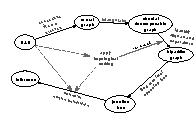
\includegraphics[width=0.9\textwidth]{img/jt_roadmap_nojust}%
	 }}
	 \only<2>{
	 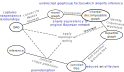
\includegraphics[width=0.9\textwidth]{img/jt_roadmap}%
	 }
	 \notesonly{
	 \caption{A road to efficient inference and a handwavy justification for the different steps}%
	 }
\end{figure}

\end{frame}

\subsection{Constructing Bayesian Networks}

\begin{frame} \frametitle{\subsubsecname}

	\begin{figure}[h]
		 \centering
		 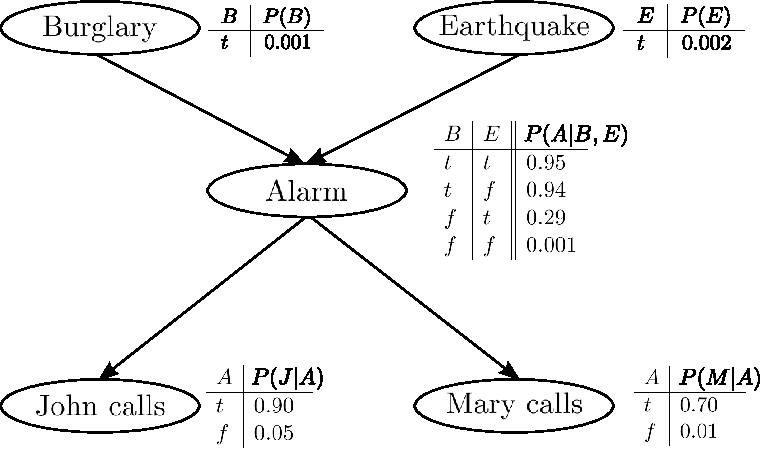
\includegraphics[width=0.5\textwidth]{img/section3_fig5_v2_2}%
		 \caption{DAG of the Californian example}
	\end{figure}
	
%	\only<2>{
%	\begin{itemize}
%		\item set of random variables 
%			$\leadsto$ nodes of the graph
%		\item direct influences between variables 
%			$\leadsto$ directed links between nodes
%		\item nodes $x_i$ are annotated with the conditional probabilities\\
%			\quad$P\big(X_i\,|\, \text{parents}(X_i)\big)$
%	\end{itemize}
%	} 
Considering statistical dependencies, only 10 instead of 31 entries have to be stored.
	{ \small
		\begin{align} 
			P(J,M,A,B,E) \stackrel{\substack{\text{product}\\\text{rule}}}{=}& 
			P(J|M,A,B,E) \, P(M|A,B,E) \, P(A|B,E) \, P(B|E) \, P(E) \\\slidesonly{\vspace{-5mm}}
			\stackrel{\substack{\text{cond.}\\\text{indep.}}}{=}& P(J|A) \, P(M|A) \, P(A|B,E) \, P(B) \, P(E)
		\end{align}
	}
\end{frame}

\begin{frame}\frametitle{\secname}
  
Bayesian Networks are a factorization of the full joint distribution\footnote{See Ch. 14 from \citep{russell2016artificial} for more details.}:

\begin{equation}
P(X_{1},\ldots,X_{n}) = \prod_{i=1}^{n} P(X_{i} | parents(X_{i}))
\end{equation}
    
\begin{itemize}
\item We only need to condition on the direct parents of any node $X_i$

\pause 
\item The factorization enables us to construct the \emph{directed acyclic graph} (DAG).
\item We can also use the DAG to formulate the factorization.
\end{itemize}

\begin{equation}
\mathit{DAG}_{\text{Bayes.Net}} \quad \corresponds \quad \prod_{i=1}^{n} P(X_{i} | parents(X_{i}))
\end{equation}
    
\end{frame}

\subsection{The Junction tree algorithm}

\begin{frame}\frametitle{\subsecname}

We need a representation that scales well for large DAGs to perform marginalization (``summing out'') and conditioning more efficiently.

The Junction tree algorithm converts into a tree structure made up of \emph{cliques} and \emph{separators}.

\question{What is a difference between a DAG and a tree?}

\pause

- A tree structure guarantees that the path between any two nodes is unique.

\end{frame}

\begin{frame} \frametitle{Trees}
	\begin{itemize}
	\item\textbf{tree}: graph where each existing path 
			between nodes is \emph{unique}
	
	\vspace{2mm}
	\begin{center}
	\begin{tabular}{cc}
		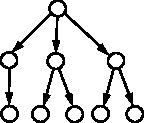
\includegraphics[width=4cm]{img/tree_directed}
		&
		\hspace{-5mm}
		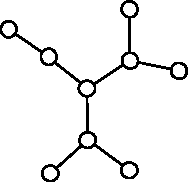
\includegraphics[width=5cm]{img/tree_undirected} \\
		directed tree & \hspace{-5mm} undirected tree 
	\end{tabular}
	\end{center}
	\end{itemize}
\end{frame}

\subsection{Decomposable Undirected Graphs}

\mode<presentation>{
\begin{frame} 
    \begin{center} \huge
        \subsecname
    \end{center}
    \begin{figure}[h]
	 \centering
	 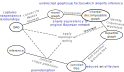
\includegraphics[width=0.8\textwidth]{img/jt_roadmap}%
	\end{figure}
    %\begin{center}   
		%\begin{align*}
		%\text{DAG}
		%\longrightarrow \substack{\text{moral}\\\text{graph}}
		%\longrightarrow \substack{\text{\textcolor{blue}{decomposable}}\\\text{\textcolor{blue}{graph}}}
		%\longrightarrow \substack{\text{bipartite}\\\text{graph}}
		%\longrightarrow \substack{\text{Junction}\\\text{Tree}}
		%\end{align*}
    %\end{center}
\end{frame}
}

% -----------------------------------------------------------------------------
\begin{frame} \frametitle{Undirected Graph}
\begin{figure}
	\centering
	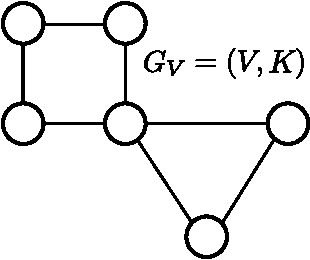
\includegraphics[width=4cm]{img/section3_fig9}
	 \caption{undirected graph \ensuremath{G_V} with vertices \ensuremath{V} and edges \ensuremath{K}} 
\end{figure}
\end{frame}

\mode<article>{
Separate $G$ (undirected graph) into two separate subgraphs $G_A$ and $G_B$
,
such that node $C$ lies on the path between \underline{any} node in $G_A$ and \underline{any} other node in $G_B$. 

\textbf{Remark}:
$C$ can also be a set of nodes (cf. ).
}

\subsubsection{Cliques and separators}

% -----------------------------------------------------------------------------
\begin{frame} \frametitle{Separators}

\only<1>{
\mode<presentation>{
	\begin{figure}
	\centering
	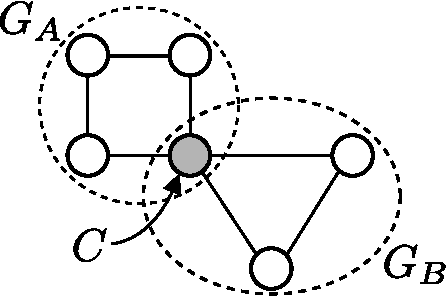
\includegraphics[width=5cm]{img/section3_fig10}
	\notesonly{\caption}\slidesonly{\caption*}{node C separates subsets A and B} 
	\end{figure}
}
}
\only<2>{
\begin{figure}[h]
     \centering
     \savebox{\imagebox}{
	 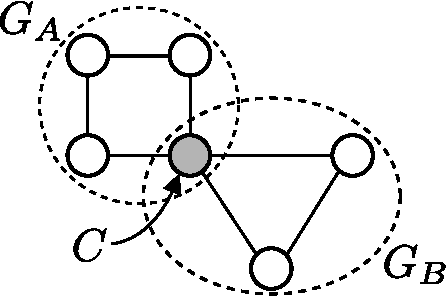
\includegraphics[width=0.4\textwidth]{img/section3_fig10}}%
     \begin{subfigure}[t]{0.35\textwidth}
         \centering
         \usebox{\imagebox}% Place largest image
         \caption{node C}
         \label{fig:nodes}
     \end{subfigure}
     \hspace{3mm}
     \begin{subfigure}[t]{0.4\textwidth}
         \centering
         \raisebox{\dimexpr.5\ht\imagebox-.5\height}{% Raise smaller image into place
         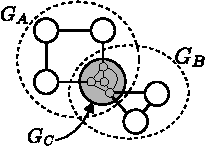
\includegraphics[width=0.95\textwidth]{img/section3_fig10_cset}
         }
         \caption{set of nodes C}
         \label{fig:setc}
     \end{subfigure}
     \caption{subgraphs A and B separated by C}
	 \label{fig:regression}
\end{figure}
}
	\slidesonly{\vspace{-2mm}}
	\begin{block}{Separator}
		A set $C$ of nodes \textbf{separates} two undirected subgraphs $G_A$ and $G_B$ 
		if \emph{every} path from node set $A$ to node set $B$ 
		has to pass through an element of $C$.
	\end{block}
\end{frame}

\subsubsection{Decomposable graphs}

% -----------------------------------------------------------------------------
\begin{frame}{Only} \frametitle{\subsubsecname}
	\vspace{-2mm}
	\begingroup
	\slidesonly{\footnotesize}
	\begin{itemize}
		\item $A,B,C$ are a \textbf{proper decomposition} 
			of an undirected graph $G = (V,K)$ if:
	%\slidesonly{\vspace{-4mm}}
			\begin{itemize}
				\item $A,B,C$ are non-empty and 
					disjoint subsets with $V=A \cup B \cup C$,
				\item $C$ separates $G_A$ and $G_B$, and
				\item subgraph $G_C$ is complete.
			\end{itemize}
		\item $G$ is \textbf{decomposable} if it is complete, 
			or a proper decomposition $A,B,C$ exist,
			\underline{where} $G_{A\cup C}$ and $G_{B \cup C}$ are decomposable.
	\end{itemize}
	\endgroup
	
	\slidesonly{\vspace{-4mm}}
	
	\pause
	
	\question{Are the following (i) a proper decomposition, (ii) decomposable graphs? \notesonly{(cf. \figref{fig:decompex1}, \figref{fig:decompex2}, \figref{fig:propernotdecompexample} and \figref{fig:propernotdecompexample4})} }

	\slidesonly{\vspace{-9mm}}
	
	\begin{enumerate}
	\item<only@2,3>[]
		%\begin{figure}[h]
		\begin{center}
		%\centering
		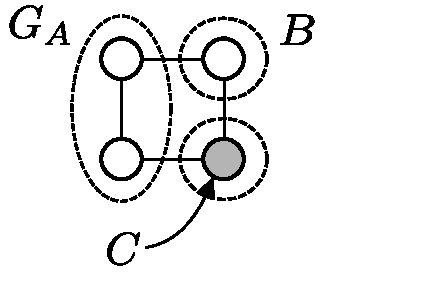
\includegraphics[width=5cm]{img/section3_fig10_sub}
		\only<3>{\captionof{figure}{not a proper decomposition \notesonly{\\}and not decomposable}
		}
		\label{fig:decompex1}
		\end{center}
	\item<only@4,5>[]
		%\begin{figure}[h]
		%\centering
		\begin{center}
		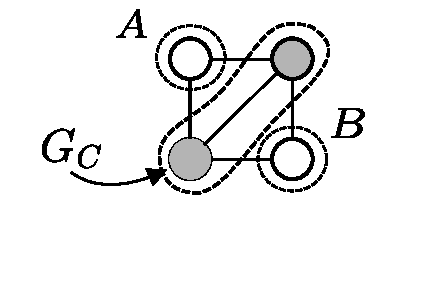
\includegraphics[width=5cm]{img/section3_fig10_sub_2}
		\only<5>{\captionof{figure}{a proper decomposition\notesonly{\\} and decomposable}
		}
		\label{fig:decompex2}
		%\end{figure}
		\end{center}
	\item<only@6,7>[]
	
		\begin{figure}[h]
		 \centering
		 \savebox{\imagebox}{
		 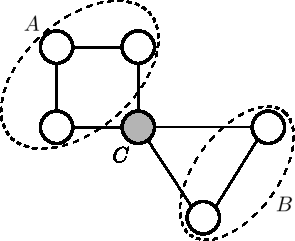
\includegraphics[width=0.3\textwidth]{img/section3_fig12}}%
		 \begin{subfigure}[t]{0.35\textwidth}
			 \centering
			 \usebox{\imagebox}% Place largest image
			 \caption{example decomposition}
			 \label{fig:propernotdecompgraph}
		 \end{subfigure}
		 \hspace{7mm}
		 \begin{subfigure}[t]{0.3\textwidth}
			 \centering
			 \raisebox{\dimexpr.5\ht\imagebox-.5\height}{% Raise smaller image into place
			 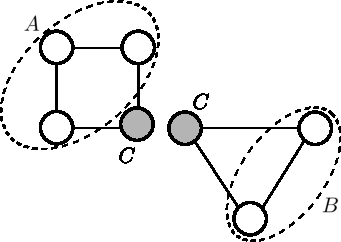
\includegraphics[width=0.99\textwidth]{img/section3_fig12_v2}
			 }
			 \caption{\underline{Hint}
			 \only<7>{: because $G_{A \cup C}$ is not decomposable}
			 }
			 \label{fig:hintnotdecomp}
		 \end{subfigure}
		 \only<7>{\caption{a proper decomposition but not decomposable}}
		 \label{fig:propernotdecompexample}
		\end{figure}
	
	\item<only@8,9>[]
	
		\begin{figure}[h]
		 \centering
		 \savebox{\imagebox}{
		 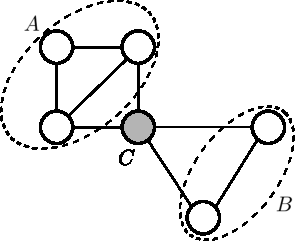
\includegraphics[width=0.3\textwidth]{img/section3_fig13}}%
		 \begin{subfigure}[t]{0.35\textwidth}
			 \centering
			 \usebox{\imagebox}% Place largest image
			 \caption{example decomposition}
			 \label{fig:propernotdecompgraph}
		 \end{subfigure}
		 \hspace{7mm}
		 \begin{subfigure}[t]{0.3\textwidth}
			 \centering
			 \raisebox{\dimexpr.5\ht\imagebox-.5\height}{% Raise smaller image into place
			 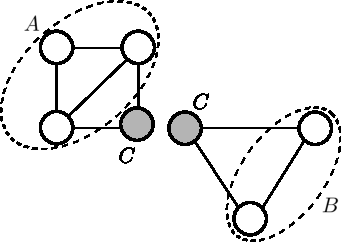
\includegraphics[width=0.99\textwidth]{img/section3_fig13_v2}
			 }
			 \caption{\underline{Hint}
			 \only<9>{: because $G_{A \cup C}$ is decomposable and $G_{B \cup C}$ is complete}
			 }
			 \label{fig:hintnotdecomp}
		 \end{subfigure}
		 \only<9>{\caption{a proper decomposition and decomposable}}
		 \label{fig:propernotdecompexample4}
		\end{figure}
	
	\end{enumerate}
	
\end{frame}

\begin{frame}\frametitle{\subsubsecname}

	\question{Why are we interested in decomposable graphs?}\\
	
	
	\pause	
	
	\slidesonly{\vspace{-10mm}}
	
	%\begin{figure}[h]
	%\centering
	%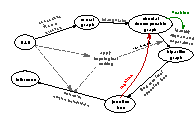
\includegraphics[height=5cm]{img/jt_roadmap_requirement}
	%\notesonly{\caption{The construction of a junction tree requires a decomposable graph of cliques.}}
	%\end{figure}
	
	\begin{figure}[h]
		 \centering
		 \hspace{-10mm}
		 \savebox{\imagebox}{
		 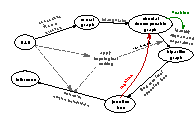
\includegraphics[width=0.5\textwidth]{img/jt_roadmap_requirement}}%
		 \begin{subfigure}[t]{0.3\textwidth}
			 \centering
			 \usebox{\imagebox}% Place largest image
		 \end{subfigure}
		 \hspace{15mm}
		 \begin{subfigure}[t]{0.35\textwidth}
			 \centering
			 \raisebox{\dimexpr.5\ht\imagebox-.5\height}{% Raise smaller image into place
			 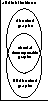
\includegraphics[width=0.3\textwidth]{img/directed_chordal_undirected_vertical}
			 }
		 \end{subfigure}
		 \mode<article>{\caption{The construction of a junction tree requires a decomposable graph of cliques.}
		 }
		\end{figure}
	
	\slidesonly{\vspace{-5mm}}
	
	
	- The short answer\notesonly{\footnote{Not required but if interested in more formal justifications see Ch 3.4 and Ch 4 from \citep{koller2009probabilistic}}}:
	\begin{enumerate}[(a)]
	\item it is a requirement for the construction of junction trees \notesonly{(cf. \sectionref{sec:constructjt})}
	\item decomposable graphs allow us to form a \emph{bipartite graph} of cliques and separators.
	\end{enumerate}
	
\end{frame}

\newpage

% -----------------------------------------------------------------------------
\begin{frame} \frametitle{\secname}

	\begin{block}{Cliques and separators}
	\begin{itemize}
		\item \textbf{cliques} are \underline{maximally complete subgraphs}
		\item decomposable graphs can be decomposed into cliques and separators
		\item cliques and separators form a \emph{bipartite graph} (cf. \figref{fig:cliquessepformbipartite})
	\end{itemize}
	\end{block}
	
	\slidesonly{\vspace{4mm}}
	
	%\begin{figure}[h]
	{
	\centering
	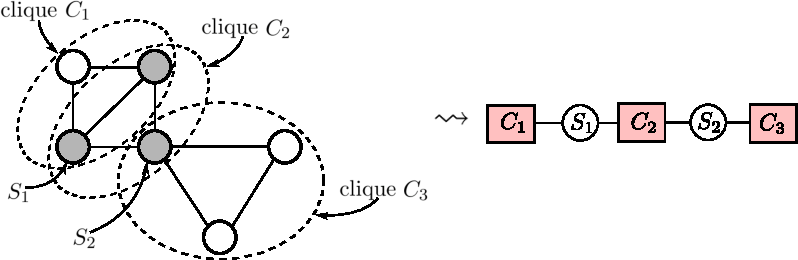
\includegraphics[height=3.5cm]{img/section3_fig15}
	\captionof{figure}{a decomposable graph and corresponding bipartite graph}
	\label{fig:cliquessepformbipartite}
	%\end{figure
	}
	
		
\end{frame}


\begin{frame}\frametitle{\subsubsecname}

\only<1>{
\mode<presentation>{
		\begin{figure}[h]
		 \centering
		 \savebox{\imagebox}{
		 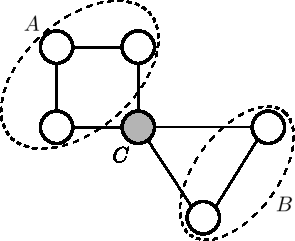
\includegraphics[width=0.3\textwidth]{img/section3_fig12}}%
		 \begin{subfigure}[t]{0.35\textwidth}
			 \centering
			 \usebox{\imagebox}% Place largest image
			 \caption{example decomposition}
		 \end{subfigure}
		 \hspace{7mm}
		 \begin{subfigure}[t]{0.3\textwidth}
			 \centering
			 \raisebox{\dimexpr.5\ht\imagebox-.5\height}{% Raise smaller image into place
			 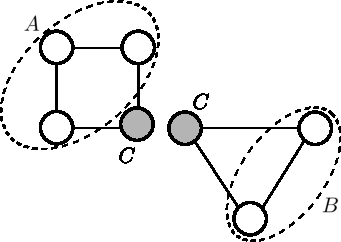
\includegraphics[width=0.99\textwidth]{img/section3_fig12_v2}
			 }
			 \caption{because $G_{A \cup C}$ is not decomposable}
		 \end{subfigure}
		 \caption{a proper decomposition but not decomposable}
		\end{figure}
}
}
	

	\question{What if we don't have a decomposable graph \notesonly{as in \figref{fig:propernotdecompexample}}?}\\
	
	\pause 
	
	- We apply triangulation. We add a \emph{chord}, i.e. ``shortcut'' edges to eliminate any ``circles'' (i.e. cycles) of 4+ vertices.
	
	\pause 
	
	According to Ch 9.4.3 in \citep{koller2009probabilistic}, constructing the \emph{chordal graph} is actually a heuristic of elimination ordering. It plays a role in keeping the size of cliques small. Smaller cliques allow for a more ``modular'' bipartite graph which leads to faster computation during inference.
	
\end{frame}

